 \documentclass[a4paper,12pt]{article}
%%%%%%%%%%%%%%%%%%%%%%%%%%%%%%%%%%%%%%%%%%%%%%%%%%%%%%%%%%%%%%%%%%%%%%%%%%%%%%%%%%%%%%%%%%%%%%%%%%%%%%%%%%%%%%%%%%%%%%%%%%%%%%%%%%%%%%%%%%%%%%%%%%%%%%%%%%%%%%%%%%%%%%%%%%%%%%%%%%%%%%%%%%%%%%%%%%%%%%%%%%%%%%%%%%%%%%%%%%%%%%%%%%%%%%%%%%%%%%%%%%%%%%%%%%%%
\usepackage{eurosym}
\usepackage{vmargin}
\usepackage{amsmath}
\usepackage{multicol}
\usepackage{graphics}
\usepackage{epsfig}
\usepackage{framed}
\usepackage{subfigure}
\usepackage{fancyhdr}

\setcounter{MaxMatrixCols}{10}
%TCIDATA{OutputFilter=LATEX.DLL}
%TCIDATA{Version=5.00.0.2570}
%TCIDATA{<META NAME="SaveForMode" CONTENT="1">}
%TCIDATA{LastRevised=Wednesday, February 23, 2011 13:24:34}
%TCIDATA{<META NAME="GraphicsSave" CONTENT="32">}
%TCIDATA{Language=American English}

\pagestyle{fancy}
\setmarginsrb{20mm}{0mm}{20mm}{25mm}{12mm}{11mm}{0mm}{11mm}
\lhead{StatsResource} \rhead{Information Theory}

%\input{tcilatex}

\begin{document}

\Large



\noindent \textbf{Discrete memoryless channel (from last lecture)}
\begin{itemize}
\item For a DMC with ``m" inputs and ``n" outputs, the input X consists of input symbols $x_1, x_2, \ldots x_m$.
\item The probabilities of these source symbols $P(x_i)$ are assumed to be known.
\item The output Y consists of output symbols $\{y_1,y_2,\ldots, y_n \}$
\item Each possible input-to-output path is indicated along with a conditional probability $P(y_j|x_i)$, where $P(y_j|x_i)$  is the conditional probability of
obtaining output $y_j$ given that the input is $x_i$. \item $P(y_j|x_i)$ is called a \textbf{\emph{channel transition probability}}.
\end{itemize}

%\end{document}
%--------------------------------------------------------%
%--------------------------------------------------------%

\noindent \textbf{Discrete memoryless channel}
\begin{itemize}
\item On the next slide, we present a binary DMC, with the channel transition probabilities indicated.
\item $P(y_1|x_1)$ = 0.9  and $P(y_2|x_1)$ = 0.1
\item $P(y_1|x_2)$ = 0.2  and $P(y_2|x_2)$ = 0.8
\end{itemize}



\begin{center}
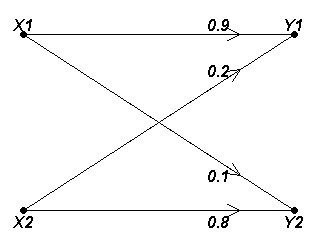
\includegraphics[scale=0.54]{10Bnet2}
\end{center}


A channel is completely specified by the complete set of transition probabilities. Accordingly, a
channel is specified by the matrix of transition probabilities $[P(Y|X)]$, given by

\[  [P(Y|X)]  = \left[ \begin{array}{cccc}
P(y_1|x_1) & P(y_2|x_1) & \ldots & P(y_n|x_1) \\
P(y_1|x_2) & P(y_2|x_2) & \ldots & P(y_n|x_2) \\
\ldots & \ldots & \ldots & \ldots \\
P(y_1|x_m) & P(y_2|x_m) & \ldots & P(y_n|x_n) \\
\end{array} \right] \]


The matrix $[P(Y|X)]$ is called the \textbf{\emph{channel matrix}}.
%ZP(yylx;) : l lor all 1 (10.12)
 

\begin{itemize}
\item Since each input to the channel results in some
output, each row of the channel matrix must sum to unity (i.e. all rows must add up to 1. This condition is not necessary for columns).
\item For the binary DMC presented previously, the channel matrix is
\[  [P(Y|X)]  = \left[ \begin{array}{cc}
0.9 & 0.1  \\
0.2 & 0.8 \\
\end{array} \right] \]
%\item (Remark: This is not a binary symmetric channel (relevant to later material))
\end{itemize}


\begin{itemize}
\item The input probabilities $P(X)$ are represented by the row matrix
\[  [P(X)]  = \left[ \begin{array}{cccc}
P(x_1) & P(x_2) & \ldots & P(x_m) \\
\end{array} \right] \]
\item The output probabilities $P(Y)$ are represented by the row matrix
\[  [P(Y)]  = \left[ \begin{array}{cccc}
P(y_1) & P(y_2) & \ldots & P(y_n) \\
\end{array} \right] \]
\item We can compute $[P(Y)] $ by the following formula: $[P(Y)]  = [P(X)]\times [P(Y|X)]$
\item (Note: Be mindful of the dimensions of each matrix).
\end{itemize}


\begin{itemize}
\item Suppose for our Binary DMC that the input probabilities were given by $[P(X)] = [ 0.5\mbox{   }0.5]$.
\item Compute $[P(Y)]$, given the channel matrix given in previous slides.
\[  [P(Y)]  =  \left[ \begin{array}{cc}
0.5 & 0.5 \\
\end{array} \right] \times \left[ \begin{array}{cc}
0.9 & 0.1  \\
0.2 & 0.8 \\
\end{array} \right] \]

\item Solving
\[  [P(Y)]  =  \left[ \begin{array}{cc}
(0.5 \times 0.9)+(0.5 \times 0.2) & (0.5 \times 0.1)+(0.5 \times 0.8) \\
\end{array} \right]  \]

\item Simplifying \[  [P(Y)]  =  \left[ \begin{array}{cc}
0.55 & 0.45 \\
\end{array} \right]  \]
\end{itemize}





\begin{itemize}
\item Let $[P(X)]$ is presented as a diagonal matrix , i.e.

\[  [P(X)]_d  = \left[ \begin{array}{cccc}
P(x_1) &0 & \ldots & 0 \\
0 & P(x_2)& \ldots & 0 \\
\ldots & \ldots & \ldots & \ldots \\
0& 0 & \ldots & P(x_m) \\
\end{array} \right] \]
\item The \emph{\textbf{ joint probability matrix}} $[P(X,Y)]$can be computed as
$[P(X,Y)]  = [P(X)]_d\times [P(Y|X)]$
\end{itemize}


\begin{itemize}
\item For the Binary DMC described in the previous example, compute the joint probability matrix.
\item Diagonalize the input probabilities for $X$.
\[  [P(X)]_d  = \left[ \begin{array}{cc}
0.5 & 0.0  \\
0.0 & 0.5\\
\end{array} \right] \]

\item Simplifying
\[  [P(X,Y)]  =  \left[ \begin{array}{cc}
(0.5 \times 0.9)+(0 \times 0.2) & (0.5 \times 0.1)+(0 \times 0.8) \\
(0 \times 0.9)+(0.5 \times 0.2) & (0 \times 0.1)+(0.5 \times 0.8) \\
\end{array} \right]  \]


\item Solving
\[  [P(X,Y)]  =  \left[ \begin{array}{cc}
0.45 & 0.05 \\
0.1  & 0.4 \\
\end{array} \right]  \]
\end{itemize}




\end{document}